\documentclass[sigconf,review,anonymous]{acmart}

%% \BibTeX command to typeset BibTeX logo in the docs
\AtBeginDocument{%
  \providecommand\BibTeX{{%
    Bib\TeX}}}

\usepackage[utf8]{inputenc}
\usepackage{amsmath, amssymb, amsfonts, colortbl, xspace, paralist, multirow, hyperref, pgfplots, booktabs, multirow}
\pgfplotsset{compat=newest}
\hypersetup{
   colorlinks=false,
   pdfborder={0 0 0},
 }
 
%~ \usepackage[disable]{todonotes}
\usepackage{todonotes}
\newcommand{\rev}[1]{{\color{blue}{#1}}}

%~ \usepackage[english]{babel}
\usepackage{graphicx, color, amssymb, url, xcolor, tikz, pgf, float, subcaption, algorithm,  tabularx}
\usepackage[noend]{algpseudocode}
\usetikzlibrary{trees, shapes, calc, external, fit, arrows, decorations, decorations.pathreplacing, patterns, automata, positioning, arrows.meta, intersections, calligraphy}


% Custom commands
\algnewcommand\algorithmicforeach{\textbf{for each}}
\algdef{S}[FOR]{ForEach}[1]{\algorithmicforeach\ #1\ \algorithmicdo}
\renewcommand{\algorithmicrequire}{\textbf{Input:}}
\renewcommand{\algorithmicensure}{\textbf{Output:}}
\newcommand{\Node}[1]{\ensuremath{\mathrm{Node}_{#1}}\xspace}
\newcommand{\flow}[1]{\ensuremath{\mathit{flow}_{#1}}\xspace}
\newcommand{\file}{\ensuremath{\mathit{File}}\xspace}
\newcommand{\storage}{\ensuremath{\mathit{Storage}}\xspace}
\newcommand{\size}{\ensuremath{\mathit{Size}}\xspace}
\newcommand{\memory}{\ensuremath{\mathit{M}}\xspace}
\newcommand{\duration}{\mathit{Duration}\xspace}
\newcommand{\bandwidth}{\mathit{Bandwidth}\xspace}
\newcommand{\core}{\mathit{Cores}\xspace}
\newcommand{\submissiontime}{\mathit{SubTime}\xspace}
\newcommand{\emptyflow}{\mathit{ReferenceFlow}\xspace}
\newcommand{\walltime}{\mathit{WallTime}\xspace}
\newcommand{\completiontime}{\mathit{CompletionTime}\xspace}
\newcommand{\start}{\mathit{StartTime}\xspace}
\newcommand{\allocatednode}{\ensuremath\mathit{\sigma}\xspace}
\newcommand{\allocatedcores}{\ensuremath\mathit{\gamma}\xspace}
\newcommand{\fileset}{\ensuremath{\mathbb{F}}\xspace}
\newcommand{\jobset}{\ensuremath{\mathbb{J}}\xspace}
\newcommand{\nodeset}{\ensuremath{\mathbb{N}}\xspace}
\newcommand{\evict}{\ensuremath{\mathcal{V}}\xspace}
\newcommand{\nbloads}{\ensuremath{\mathit{\mathit{Loads}}}\xspace}
\newcommand{\live}{\ensuremath{L}\xspace}
\newcommand{\us}{\ensuremath{\mathit{user~session}}\xspace}
\renewcommand{\algorithmicrequire}{\textbf{Input:}}
\renewcommand{\algorithmicensure}{\textbf{Output:}}

\begin{document}

\title{Locality-aware batch scheduling of I/O intensive workloads}

\begin{abstract}
  Clusters make use of workload schedulers such as
  the Slurm Workload Manager to allocate computing jobs onto
  nodes. These schedulers usually aim at a good trade-off between
  increasing resource utilization and user satisfaction (decreasing
  job waiting time). However, these schedulers are typically unaware
  of jobs sharing large input files, which may happen in data
  intensive scenarios. The same input files may be loaded several
  times, leading to a waste of resources.
   
  We study how to design a \textit{data-aware job scheduler} that is
  able to keep large input files on the computing nodes, without
  impacting other memory needs, and can use previously loaded files to
  \textit{limit data transfers in order to reduce the waiting times of
    jobs}.

  We present three schedulers capable of distributing the load between
  the computing nodes as well as re-using an input file already loaded
  in the memory of some node as much as possible.
  
  We perform simulations using real cluster usage traces to compare
  them to classical job schedulers.  The results show that
  keeping data in local memory between successive jobs and using data
  locality information to schedule jobs allows a reduction in job
  waiting time and a drastic decrease in the amount of data transfers.

  %%%% Longer version below:
  %   Clusters and supercomputers make use of workload schedulers such as
  % the Slurm Workload Manager or OAR to allocate computing jobs onto nodes. These schedulers
  % usually aim at a good trade-off between increasing resource
  % utilization and user satisfaction (decreasing job waiting
  % time). However, these schedulers are typically unaware of jobs
  % sharing large input files: in data-intensive scenarios, tens to
  % hundreds of jobs dedicated to the study of the same multi-GB input
  % file may be successively submitted. Running each of these jobs
  % first requires to load the input file, leading to a large data
  % transfer overhead. Users could manually group some of these
  % tasks into larger jobs to reduce data transfers, but this would result in less granular units that are
  % more difficult to schedule by the resource manager, and would
  % thus result in a larger delay as well. We study how to design a \textit{data-aware
  %   job scheduler} that is able to keep large input files on the 
  % computing nodes, provided this does not impact the memory needs of
  % other jobs, and can use previously loaded files to \textit{limit
  %   data transfers in order to reduce the waiting times of jobs}.

  % We present three schedulers capable of distributing the load between
  % the computing nodes as well as being aware of what the memory of each
  % node contains in order to re-use an input file
  % already loaded in the memory of some node as many times as possible.
  
  % We report simulations performed using real cluster usage traces. 
  % Our approach is compared to currently used schedulers in batch systems.
  % The results show that keeping data locally, in memory, between successive
  % jobs and using data locality information to schedule jobs allows a
  % reduction in job waiting time and a drastic decrease in the amount of data
  % transfers.

\end{abstract}

\maketitle

\keywords{
%~ Batch scheduling,
Job input sharing,
%~ Real workload,
Data-aware,
Job scheduling,
High Performance Data Analytics
%~ Job-input-aware
%~ Communication-aware,
%~ Batch systems
}
\section{Introduction}\label{sec.introduction}

To meet the ever-increasing demand for scientific computation power,
High-Performance Computing platforms are typically composed of large
numbers of computation nodes. Scientists typically submit their
computation jobs to a scheduler, which decides the ordering and mapping
of the jobs on the platform. This needs to be performed with particular
care of balancing between resource utilization and user satisfaction, so
as to leverage the computation resources as efficiently as possible,
while avoiding adverse pathological cases that could particularly impact
some users rather than others.

Computation jobs however need data input which, more often than not, can
be very large, notably for many subfields of life science with highly
data-dependent workflows \rev{like taxonomic identification of DNA fragments, genome alignments or ancestral reconstructions}.
Loading such data input from the storage
nodes may consume a significant part of the job duration. This load
penalty can however be avoided altogether when the data was actually
already used by the previous job running on the computation node, and
thus still immediately available on the node. Taking care of scheduling
jobs that use the same data input one after the other thus allows to
reduce the jobs completion times, leading to better platform usage
efficiency. Unfortunately, classical job schedulers mostly do not take
data input into account, and thus do not benefit from such data reuse ;
most jobs always have to re-load their data input.

In this paper, we propose to model the benefits of re-using data loads
between successive jobs, and we introduce new algorithms that add such
data reuse to the scheduling balance. By tracking which data is loaded
on which node for the scheduled jobs, they are able to significantly
reduce data loads, thus improving both resource utilization and user
satisfaction. We evaluated these algorithms thanks to traces of actual
jobs submissions observed on a large cluster platform. This allows to
assess the effectiveness of our heuristics over a variety of realistic
working sets. This revealed that while our heuristics get slightly worse
results over some working set samples (those which exhibit cluster ample
underuse), most working set samples largely benefit from our heuristics,
leading to interesting benefit overall.

We thus present the following contributions in this paper:
\begin{itemize}
	\item We formalize our model of scheduling data-intensive jobs sharing input files on a cluster (Section~\ref{sec.framework}).
	\item We propose three new schedulers focusing on re-using input files while minimizing evictions and avoiding starvation (Section~\ref{sec.schedulers}).
	\item We extract job information from historical logs of a cluster to build workloads that correspond to the needs and behaviors of real users (Section~\ref{sec.working}).
	\item We implement all three heuristics as well as two state-of-the-art schedulers on a simulator and study the performance (mean stretch, amount of time spent waiting for a file to be loaded \rev{and number of core hours}) obtained \rev{after scheduling almost 2 millions jobs} (Section~\ref{sec.evaluations}).
	Our evaluation demonstrate that our heuristics in most cases surpass the state of the art schedulers.
	We show that workloads that heavily saturate the cluster
    benefits much more from our strategies which results
    considerable reduction in the job waiting times \rev{as well as the total core hours}.
\end{itemize}

\section{Related work}\label{sec.related_work}

\subsection{Scheduling jobs on large clusters}

A various number of workloads managers have emerged 
as a way to meet the rising numbers of high performance computing clusters.
Workload managers like Slurm~\cite{SLURM}, OAR~\cite{oar},
TORQUE~\cite{torque}, LoadLeveler~\cite{loadleveler},
Portable Batch System~\cite{pbs}, SunGrid~\cite{sungrid}
or Load Sharing Facility~\cite{lsf} all offer
various scheduling strategies.

The First-Come-First-Served (FCFS) algorithm is the prevalent default
scheduler on most of these solutions~\cite{survey_workload_manager_and_scheduler}.
Moreover, Slurm is used on most of the TOP500 supercomputers and its default strategy is FCFS~\cite{slurm_website_scheduling} as well.
A backfilling strategy is known to increase
the use of supercomputer resources~\cite{maui}~\cite{New_Backfill}. 
The most commonly used backfilling strategy, called conservative 
backfilling~\cite{Characterization_of_Backfilling}~\cite{Introducing-New-Backfill-based} follows
a simple paradigm: "a job can only be backfilled if it does not
delay a job of higher priority".
We can then safely assume that comparing ourselves to FCFS with and without conservative backfilling can 
bring significant insights on what improvements can be achieved on data-intensive workloads.

Other scheduling strategies exist like 
Maui~\cite{Maui_Scheduler}, Gang scheduling~\cite{gang_scheduling}, 
RASA~\cite{rasa} that use the advantages of both Min-min and Max-min algorithms,
RSDC~\cite{rsdc} that divides large jobs in sub jobs for a more refined scheduling,
or PJSC~\cite{pjsc} and PSP+AC~\cite{PSP_AC} that are a priority-based schedulers; 
however these heuristics do not consider the impact
input re-use could have on data-intensive workloads.
We aim at resolving this issue in this paper.

\subsection{Using distributed file systems to deal with data-intensive workloads}

Distributed file systems are a solution to ease the access to 
shared input files. They facilitate the execution of I/O-intensive batch
jobs by selecting appropriate storage policies.

Batch-Aware Distributed File System~\cite{Explicit_Control_in_a_Batch-Aware_Distributed_File_System},
is designed to orchestrate large, I/O-intensive batch workloads on remote computing clusters.
HDFS~\cite{hdfs} (Hadoop Distributed File System)
incorporates storage-aware scheduling. 
%It is particularly used to store large volumes of data on a large number of systems.
It migrates a computation closer to where the data is
located, rather than moving the data to where the application is
running, in order to reduce communication.
%~ HDFS is mainly a storage system, thus it uses an historic on files locations to serve as a backup. 

These solutions are mainly storage systems that uses a history of file locations to serve as a backup.
In our scenario, we copy the data from an already-redundant system (an online database for example)
and store it locally on the node in an ephemeral way.
Thus, in the event of a crash, we do not manage the data which is already redundant, it simply results in an aborted job.
Secondly, the scheduling can cause issues. Weets et al. describe some problems from
MapReduce~\cite{issue_with_hdfs}, the programming model used in HDFS, in detail.
By not using HDFS or any distributed file system, we avoid these problems altogether. 
Lastly, file systems are particularly efficient when the input data used are identical over time.
In our case, between users, the inputs will be largely different, making distributed file systems less efficient.


%~ However, the main idea is not data re-use, but to
%~ facilitate the execution of I/O intensive batch
%~ jobs by selecting appropriate storage policies
%~ in regards to I/O scoping (creating a custom environment for each job
%~ for data that will be used a lot by the job, thus not accessing the main disk too
%~ much) and space allocation.


\subsection{Using schedulers to deal with data-intensive workloads}

Some schedulers tackle the issue of data-intensive workloads. 
A solution can be to minimize network contention by allocating nodes to even out node and
switch contention~\cite{minimize_network_contention}. 
In our model, we are not studying the network topology and consider independent nodes.
This is reasonable, since our main concern is the cross-section bandwidth to a shared storage solution.
%~ Moreover, this requires a tree-based network topologies, which is different from our model.
%~ Furthermore, we are scheduling further down the topology (i.e nodes and not switches).
%
Nikolopoulos et al.~\cite{Nikolopoulos2003AdaptiveSU}
focus on a better utilization of idling memory together with 
thrashing limitation.
Our focus will be to control data loads in order to limit eviction
and will thus naturally limit thrashing. 
%
Agrawal et al.~\cite{Scheduling_Shared_Scans_of_Large_Data_Files}
propose to schedule jobs not sharing a file first
and to use a stochastic model of job arrivals for each input file to maximize re-use.
This work is aimed at the Map-Reduce model and allows to predict future jobs arrivals, two prerequisites that we do not consider. 
%
Equipping each node with a scheduler that follows a work
stealing strategy in order to manage both data locality 
and load balancing is also a solution to reduce data transfers~\cite{Optimizing_load_balancing_and_data_locality_with_data_aware_scheduling}. 
%
Selvarani et al. propose an improved activity-based costing scheduler~\cite{Improved_cost_based_algorithm}
% where the scheduler adapt itself to different application types (CPU intensive, needing high memory, large I/O cost), but our focus will be more generic and aim at maximizing data re-use to meet these needs.
where the processing capacity of each resource is evaluated to make the right decision.
Our approach is more focused on maximizing data re-use on a 
set of identical nodes.

%~ An interesting solution proposed in the context
%~ of the Jacobi-Davidson implementation for solving large
%~ eigenproblems~\cite{loadbalance_and_trashing} tackle both load balancing and memory constraint. For the load balancing, they 
%~ estimate the time needed by the fastest processor to perform the required $m$ jobs. Thus they can equilibrate the load
%~ with this information. In our study we could use a similar strategy by estimating the 
%~ processing time of a job, the length of a file transfer, and the amount of file transfers needed.
%~ To deal with memory constraint the strategy applied in the paper is to check if 
%~ nodes are thrashing data. If yes, it will recede execution of jobs on this node.
%~ The main differences are that they are using dynamic jobs. Also, we would like to 
%~ manage eviction and optimize data reuse during the scheduling phase, instead of
%~ receding execution on nodes.
%~ But is specific to the Jacobi-Davidson method

\section{Framework}\label{sec.framework}

We consider the problem of scheduling a set of $N$ independent jobs,
denoted $\jobset = \{J_1, J_2, \ldots, J_N\}$ on a set of $P$ nodes:
$\nodeset = \{\Node{1}, \Node{2}, \\ \ldots, \Node{P}\}$.
%% LM: to be merged later:
Each node $\Node{i}$ is equipped with $m$ cores noted:
$c^i_1,\ldots,c^i_m$ sharing a memory of size $\memory$.

Each job depends on an input file noted $\file(J_i)$, which is
initially stored in the main shared file system.  During the
processing of a job $J_i$ on $\Node{k}$, file $\file(J_i)$ must be in
the memory of $\Node{k}$. If this is not the case before starting
computation of job $J_i$, then file $\file(J_i)$ is loaded into the
memory.  We denote by $\fileset = \{F_1, F_2, \ldots, F_n\}$ the set
of distinct input files, whose size is denoted by $\size(F_i)$. Each
job runs on a single node, but on different numbers of cores.



Each job $J_i$ has the following attributes:
\begin{itemize}
\item Resource requirement: job $J_i$ requests $\core(J_i)$  cores, such that $1 \leq \core(J_i) \leq m$;
\item Input file: $\file(J_i) \in \fileset$;
\item Submission date: $\submissiontime(J_i)$;
\item Requested running time (or walltime): $\walltime(J_i)$: if not
  finished after this duration, job $J_i$ is killed by the scheduler;
\item Actual running time: $\duration(J_i)$ (unknown to  the scheduler
  before the job completion).
\end{itemize}

We do not consider the data output of jobs.
Each of the $N$ jobs must be processed on one of the $P$ nodes.  As
stated earlier, the shared file system initially contains all files
in $\fileset$.  Each node is connected to the file system with a link
of limited bandwidth, denoted by $\bandwidth$: transferring a data of
size $S$ from the shared file system to some node's memory takes a
time $S/\bandwidth$.
The limited bandwidth
as well as the large file sizes are the reasons why we aim at
restricting the amount of data movement.

We consider that the memory of a node, denoted by
$\memory$ is only used by the jobs' input files, since all other data are
negligible compared with the input files. We assume that jobs are
devoted a fraction of the memory proportional to the number of
requested cores, so that jobs willing to process large input files
must request large number of cores. This way, we make sure that the
memory of a node is large enough to accommodate all input files of running jobs.
A file stored in the memory of a node can be shared by two jobs $J_i$ and $J_j$ only in the following situations:
\begin{enumerate}
	\item $J_i$ and $J_j$ are computed in parallel on the same node.
	\item $J_i$ and $J_j$ are computed on the same node
          consecutively (i.e., no job is started on this node before the
          completion of $J_i$ and the start of $J_j$).
\end{enumerate}
This can hold true if the file data is accessed through I/O (traditional or memory-mapped),
allowing the same page cache to serve multiple processes from different jobs.
Otherwise we consider that memory operations of jobs scheduled between
$J_i$ and $J_j$ will cause the file to be evicted.

% We now more formally define the allocation of the jobs to the node and
% their schedule.
% We denote by $\storage(\Node{k}, t)$, the set of files loaded on $\Node{k}$
% at time $t$. The constraint on the limited size of the memory can be
% summarized by:
% $$
% \forall k,\forall t \quad \sum_{F_i\in \storage(\Node{k},t)}
% \size(F_i)\leq \memory.
% $$

For each job $J_i$, the scheduler is in charge of deciding which node
will process $J_i$, and more precisely which cores of this node
are allocated to the job, as well as a starting time $t_k$ for $J_i$. Job
$J_i$ is thus allocated a time window from $t_k$ to
$t_k+\walltime(J_i)$ devoted to (i) possibly loading the input file
$\file(J_i)$ in the memory (if it is not already present at time
$t_k$) and (ii) executing job $J(i)$. If the job has not completed at
time $t_k+\walltime(J_i)$, it is killed by the scheduler to ensure
that later jobs are not delayed.  The scheduler must also make sure
that no two jobs are executed simultaneously on the same cores.

It is important to note that the file transfer is done before the computation and cannot be overlapped.
Jobs are non-preemptible: when started, a job is executed through its completion.

Our objective is to reach an efficient usage of the platform and to
limit job waiting times. Each
user submitting jobs is interested in obtaining the result of jobs
as soon as possible. Hence we focus on the time spent in the system
for each job, also called the flow time (or flow) of the job:
$$
% \mathit{Flow}(J_i) = \completiontime(J_i) - \start(J_i).
\mathit{Flow}(J_i) = \completiontime(J_i) - \submissiontime(J_i).
$$

In the following, we want to consider aggregated performance metrics on
job flows, such as average flow. However, the duration
of a job significantly impacts its flow time. Jobs with the same
flow but very different durations do not experience the same quality
of service. To avoid this, the \emph{stretch} metric has been
introduced that compares the actual flow of a job to the one it would
experience on an empty cluster:
\begin{eqnarray*}
\emptyflow(J_i) &=& \duration(J_i) + \frac{\size(\file(J_i))}{\bandwidth}\\
\mathit{stretch}(J_i) &=& \frac{\mathit{Flow}(J_i)}{\emptyflow(J_i)}.
\end{eqnarray*}
The stretch represents the slow-down of a job due to sharing the
platform with other jobs. Considering the stretch
allows to better aggregate performance from small and large jobs.

\todo[inline]{Max: Do we want the macro \us for user sessions? And write it like that everywhere in the paper?}
\rev{
Finally, what is important for a user is that all the jobs he has submitted at once are finished as soon as possible.
Thus we introduce the notion of \us.
A \us is the sum of the stretch of jobs submitted by a user in a 5-minute window.
It is the stretch of each \us that is used in the figures of Section~\ref{sec.evaluations}.
}


\section{Job scheduling with input files}\label{sec.schedulers}


Here, we present various schedulers used to allocate jobs to
computing resources. We start with two reference schedulers (FCFS and EFT)
and then move to proposing three locality-aware job schedulers (named
LEA, LEO and LEM). Each of these five schedulers can be used both
without or with backfilling. For the sake of clarity, we first present
the simpler version, without backfilling, before detailing the modifications needed to including backfilling.

As presented above, the task of the scheduler is to allocate a set of
cores of one node
to each job submitted until now: some jobs may be started right away,
while other jobs may be delayed and scheduled later: resource
reservations are made for these jobs. Jobs are presented to the
scheduler in the form of a global queue, sorted by job submission
time. These scheduling policies are online algorithms which are called each time
a task completes (making cores available) or upon the submission of
a new job.
%Note that in accordance to our framework, each job is allocated to one or several cores of a single node.



% Some of these methods uses start or completion time as a way to
% schedule each job (section~\ref{subsec.fcfs_eft}) while another compute 
% a score to choose the best node (section~\ref{subsec.score}) and others
% are opting for a mixed strategy between locality and earliest possible start time
% (sections~\ref{subsec.mixed} and~\ref{subsec.opportunistic}).

\subsection{Two schedulers from the state of the art: FCFS and EFT}\label{subsec.fcfs_eft}

A widely-used job scheduler that is typically considered to be efficient is
First-Come-First-Serve (FCFS), detailed in
Algorithm~\ref{algo.fcfs}. Implementing this scheduler requires to
remember the time of next availability for each core. Then, for each job, we look
for the first time when a sufficient number of cores is available, and we allocate the job to
those cores.


\begin{algorithm}[htbp]%\small
\caption{First-Come-First-Serve (FCFS)}\label{algo.fcfs}
\begin{algorithmic}[1]
	\ForEach{$J_i \in$ the jobs queue} %\Comment{The job's queue is sorted by submission times}
        \ForEach{$\Node{k} \in \nodeset$}
        \State Find smallest time $t_k$ such that $\core(J_i)$ cores are available on \Node{k}\label{fcfs.ln.find}
        % Version with backfilling: \State Find smallest time $t_k$ such that $\core(J_i)$ cores are available until at least time $t_k + \walltime(J_i)$ on cores $c_1, ..., c_{\core(J_i)}$ of $\Node{k}$
        \EndFor
        \State Select \Node{k}  with the smallest $t_k$
        \State Schedule $J_i$ on $\core(J_i)$ cores of \Node{k} that are available starting from $t_k$
        \State Mark these cores busy until time $t_k +\walltime(J_i)$
%		\State Cores $c_1, ..., c_{\core(J_i)}$ of $\Node{k}$ are updated to be available at time $t_k + \walltime(J_i)$
%		\State Cores $c_1, ..., c_m$ of $\Node{k}$ are sorted in increasing order of available time \Comment{With a sorted list of cores, writing line 3 is easier}
	\EndFor
	\end{algorithmic}
\end{algorithm}


FCFS is a standard baseline comparison
for job scheduling. However, it is not aware of the capability of the
system to keep a large data file in the memory of a node between the execution of
two consecutive jobs.
A first step towards a locality-aware scheduler
is to select a node for each job not based on the cores' availability
time, but also using the file availability time, based on the file
transfer time. This is the purpose of the Earliest-Finish-Time (or
EFT) scheduler, described in Algorithm~\ref{algo.eft}: by selecting
the node that can effectively start the job at the earliest time, it
minimizes the job completion time. There are three scenarios to compute the
time $t'_k$ at which the input file of a job $J_i$ is available on
\Node{k}:
\begin{enumerate}
\item A job started before $J_i$ on \Node{k} uses the same input
  file and it is already in memory, thus $t'_k=t_k$;
\item The input file of $J_i$ is not in memory and
  $t'_k=t_k+\frac{\size(\file(J_i))}{\bandwidth}$;
\item The input file of $J_i$ is partially loaded on \Node{k}: this
  happens when some
  job $J_j$ using the same input file has been scheduled on other cores of
  the same node at time $\start(J_j)<t_k$ but the file transfer has not
  completed at time $t_k$. Then the file will be available at time:
  $t'_k = \start(J_j)+\frac{\size(\file(J_i))}{\bandwidth}.$
\end{enumerate}


% Under our model, a fair baseline would be a scheduler capable
% of reducing file transfers while keeping the First-Come-First-Serve
% principle. This scheduler is Earliest-Finish-Time (or EFT).
% It's an enhanced version of FCFS which chooses to schedule a job
% on the node with the earliest available finish time, thus considering
% the time to load the file, and consequently choosing nodes where a file will
% be re-used. 
% \todo[inline]{Max: Say that EFT with bf consider completion time as well.}
% \todo[inline]{Max: The large comment I added in Algo2 should maybe be in a text before with a smaller comment with a reference to the text?}
		
\begin{algorithm}[htbp]%\small
\caption{Earliest-Finish-Time (EFT)}\label{algo.eft}
\begin{algorithmic}[1]
	\ForEach{$J_i \in$ the jobs queue}
		\ForEach{$\Node{k} \in \nodeset$}
			\State Find smallest time $t_k$ such that $\core(J_i)$ cores are available \Node{k}
			% \State Find smallest time $t_k$ such that $\core(J_i)$ cores are available until at least time $t_k + \walltime(J_i)$ on cores $c_1, ..., c_{\core(J_i)}$ of $\Node{k}$
			\State Find time $t_k' \geq t_k$ at which $\file(J_i)$ is available on $\Node{k}$ %\Comment{There are 3 scenarios. 1: the file is already in memory ($t_k' = t_k$), 2: the file is absent ($t_k' = t_k + \frac{\size(\file(J_i))}{\bandwidth}$), 3: the file is partially loaded by another job $J_i'$ started before time $t_k$ ($t_k' = t_k + \frac{\size(\file(J_i))}{\bandwidth} - \bandwidth \times (t_k - \start(J_i'))$)}
		\EndFor
                \State Select \Node{k}  with the smallest $t'_k$
                \State Schedule $J_i$ on $\core(J_i)$ cores of \Node{k} that are available starting from $t_k$
                \State Mark these cores busy until time $t_k +\walltime(J_i)$
                %\State Schedule $J_i$ on the node with the smallest $t_k'$
%		\State Cores $c_1, ..., c_{\core(J_i)}$ of $\Node{k}$ are updated to be available at time $t_k + \walltime(J_i)$
%		\State Cores $c_1, ..., c_m$ of $\Node{k}$ are sorted in increasing order of available time
	\EndFor
\end{algorithmic}
\end{algorithm}

\subsection{Data-locality-based schedulers}

The previous strategies focus on starting (FCFS) or finishing (EFT) a job
as soon as possible, respectively.  Those are good methods
to avoid node starvation and reduce queue times.  However, they
may lead to loading the same input file on a large number of nodes in
the platform, only to minimize immediate queue times. Time is thus spent
loading the input file multiple times. This can affect the global
performance of the system by delaying subsequent jobs.  We present three
strategies that attempt to take data locality into account in a better way to reduce queuing times in the long run by increasing data reuse.

% When the platform is fully loaded, favoring data reuse helps reducing the number of file
% copies and hence reduces queue time in the long run.

The first proposed algorithm called Locality and Eviction Aware (LEA)
and detailed in Algorithm~\ref{algo.lea} aims at a good balance
between node availability and data locality.  We consider three
quantities to rank nodes:
\begin{itemize}
\item The availability time for computation $t_k$;
\item The time needed to complete loading the input file for the job
  on \Node{k} ($t'_k - t_k$);
\item The time required to reload files that need to be evicted before
  loading the input file; this time is computed using all files in
  memory and considering that a fraction of these files need to be
  evicted, corresponding to the fraction of the memory used by the job.
\end{itemize}

The intuition for the third criterion is that if loading a large file
in memory requires the eviction of many other files, these files will not
be available for later jobs and may have to be reloaded.
In the LEA strategy, we put a strong emphasis on data loading, in order
to really favor data locality. Hence, when computing the score for
each node \Node{k}, we sum the previous three quantities, with a weight
$W$ for the second one (loading time). In our experiments, based on
empirical evaluation, we set this value to $W=500$, incidentally roughly
equivalent to the number of nodes.
Note that the other two quantities usually have very different values:
the availability time is usually much larger than the time for
reloading evicted data. Hence this last criterion is mostly used as a
tie-break in case of equality of the first two criteria.



\begin{algorithm}[t]%\small
\caption{Locality and Eviction Aware (LEA)}\label{algo.lea}
\begin{algorithmic}[1]
	\ForEach{$J_i \in$ the jobs queue}
		\ForEach{$\Node{k} \in \nodeset$}
			\State Find smallest time $t_k$ such that $\core(J_i)$ cores are available
			% \State Find smallest time $t_k$ such that $\core(J_i)$ cores are available until at least time $t_k + \walltime(J_i)$ on cores $c_1, ..., c_{\core(J_i)}$ of $\Node{k}$
			\State Find time $t_k'\geq t_k$ at which $\file(J_i)$ is available on $\Node{k}$
			\State $\mathit{LoadOverhead} \gets t_k' - t_k$ %\Comment{It thus gets the load's duration}
%			\State Let $\mathit{sub\_J}$ be the subset of jobs that ends right before time $t_k$ on $\Node{k}$
                        \State Let $\mathcal{F}$ be the set of files in the memory of node \Node{k} at time $t_k$
			\State $\mathit{EvictionPenalty} \gets (\sum_{F_j\in\mathcal{F}}\size(F_j) \times \size(\file(J_i))/\memory)/\bandwidth$
			\State $score_{\Node{k}} \gets t_k + W \times \mathit{LoadOverhead} + \mathit{EvictionPenalty}$
		\EndFor
                \State Select \Node{k} with the smallest $score_{\Node{k}}$
                \State Schedule $J_i$ on $\core(J_i)$ cores of \Node{k} that are available starting from $t_k$
                \State Mark these cores busy until time $t_k +\walltime(J_i)$
	\EndFor
\end{algorithmic}
\end{algorithm}

%\subsection{LEO}

The LEA strategy puts a dramatic importance on data loads. Hence, it
is very useful when the platform is fully loaded and  some jobs
can safely be delayed to favor data reuse and avoid
unnecessary loads. However, when the platform is not fully loaded,
delaying jobs can be detrimental, as it can increases the response
time for some jobs, without any benefit for other jobs. Our second proposed strategy,
named Locality and Eviction Opportunistic (LEO) and described in Algorithm~\ref{algo.leo}, tries to adapt based
on the current cluster load: if we find some nodes that can process the job
right away, we select the one that will minimize the completion time
(as in the EFT strategy). Otherwise, we assume that the platform is
fully loaded and we apply the previous LEA strategy, to favor data reuse.


\begin{algorithm}[t]%\small
\caption{Locality and Eviction Opportunistic (LEO)}\label{algo.leo}
\begin{algorithmic}[1]
	\ForEach{$J_i \in$ the jobs queue}
		\ForEach{$\Node{k} \in \nodeset$}
			\State Find smallest time $t_k$ such that $\core(J_i)$ cores are available
			% \State Find smallest time $t_k$ such that $\core(J_i)$ cores are available until at least time $t_k + \walltime(J_i)$ on cores $c_1, ..., c_{\core(J_i)}$ of $\Node{k}$
			\State Find time $t_k'\geq t_k$ at which $\file(J_i)$ is available on $\Node{k}$
			\State $\mathit{LoadOverhead} \gets t_k' - t_k$ %\Comment{It thus gets the load's duration}
                        \State Let $\mathcal{F}$ be the set of files in the memory of node \Node{k} at time $t_k$
			\State $\mathit{EvictionPenalty} \gets (\sum_{F_j\in\mathcal{F}}\size(F_j) \times \size(\file(J_i))/\memory)/\bandwidth$
			\If{$t_k = \mathit{current\_time}$}
				\State $score_{\Node{k}} \gets t'_k$
			\Else
			         \State $score_{\Node{k}} \gets t_k + W \times \mathit{LoadOverhead} + \mathit{EvictionPenalty}$
			\EndIf
		\EndFor
                \State Select \Node{k} with the smallest $score_{\Node{k}}$
                \State Schedule $J_i$ on $\core(J_i)$ cores of \Node{k} that are available starting from $t_k$
                \State Mark these cores busy until time $t_k +\walltime(J_i)$
	\EndFor
\end{algorithmic}
\end{algorithm}

We present a third strategy called Locality and Eviction Mixed (LEM)
and described in Algorithm~\ref{algo.lem} that takes a similar approach to
LEO but performs a simple mix between the EFT and the LEA strategies:
when the \rev{platform is saturated (each node is running
at least one job)}, the LEA strategy is applied,
otherwise the EFT strategy is used.
 

\begin{algorithm}[htbp]%\small
\caption{Locality and Eviction Mixed (LEM)}\label{algo.lem}
\begin{algorithmic}[1]
	\ForEach{$J_i \in$ the jobs queue}
		%~ \State $\mathit{load} \gets$ percentage of nodes running at least one job at current time
		%~ \If{$\mathit{load} < 80$}
		\If{\rev{each node is running at least one job at $\mathit{current\_time}$}}
			\State $LEA(\jobset,\nodeset)$
		\Else
			\State $EFT(\jobset,\nodeset)$
		\EndIf
	\EndFor
\end{algorithmic}
\end{algorithm}



\subsection{Adding backfilling to all strategies}

As mentioned above, backfilling has been proposed to increase the
performance of job schedulers, by allowing jobs with lower priority to be
scheduled before jobs with higher priority. In our setting, the
priority is directly linked to the submission order: if $J_i$ is
submitted before $J_j$, then $J_i$ has a higher priority than $J_j$.
In order to avoid jobs
being perpetually delayed, bounds have to be set on how already-scheduled
jobs can be affected by backfilling. As discussed above,
Conservative Backfilling is the most restrictive version and one of
the most commonly-used strategies to improve cluster utilization. It
forbids any modification on the resource
reservations of high-priority jobs: a job may be scheduled
before other jobs that appear earlier in the queue, provided that it
does not impact the starting time of these jobs.


For each of the previous scheduling strategies, we consider a variant
using conservative backfilling (suffixed by -BF).  To add
backfilling, Algorithms~\ref{algo.fcfs}, \ref{algo.eft},
\ref{algo.lea} and~\ref{algo.leo} have to be modified: we change the
choice of the earliest time when resources are available for a job
(Line~\ref{fcfs.ln.find}). Instead of considering the time at which
cores are (indefinitely) available, we look for an availability time
window starting at $t_k$ long enough to hold the
job. Specifically, we change Line~\ref{fcfs.ln.find} into:
\begin{algorithmic}[0]
  \State $\ref{fcfs.ln.find}'$: Find smallest time $t_k$ such that $\core(J_i)$ cores are
  available from $t_k$ until $t_k + \walltime(J_i)$ on $\Node{k}$
\end{algorithmic}

Note that this requires the schedulers to store  the whole occupation profile of
each core (with availability and unavailability times), whereas the
version of each scheduler without backfilling simply requires the time
of last job completion on each core.

\section{Performance evaluation and analysis}\label{sec.evaluations}

\rev{
Actual workloads at HPC resources shared by a great number of users with diverse needs can contain 
%structures
%that are non-trivial to replicate in a fully artificial simulated job pattern.
%We believe that this is especially
%true for data-dependent patterns, 
%where a 
projects that might launch a burst of jobs using the same file just a few thousand
core hours in length, then be quiet for a long time processing the results, and then launch another such burst.
On our cluster, we have observed such behavior and present in this section how we replicate them.
%However
Changing the scheduling strategy of a production cluster for
scheduling research would disrupt the community using this cluster.
For this reason, we choose to perform simulations based on logs of a
real computing platform. In this section, we describe how we used
these logs as well as the results of the corresponding simulations.
%~ All strategies as well as the two baselines have been implemented on
%~ a simulator that we developed.
}

\subsection{\rev{Platform description}}
\rev{
We use a university cluster shared between several research laboratories. As mentioned above, a variety of applications including genomics analysis are performed on this cluster.
Our cluster contains 9720 cores spread over 486 nodes. Each node has two 10-core Intel Xeon V4 CPU at 2.20 GHz/core.
Most of the nodes have 128GB of RAM, and a few are larger.
To avoid an additional constraint, while maintaining a model close to the real cluster,
we consider that the platform is made of 486 homogeneous nodes of size $\memory = 128GB$.

As mentioned above, we observed the submission of IO intensive jobs on the platform we extracted the logs from. The cluster is often used
for taxonomic identification of DNA fragments. To perform such identification, the Kraken2 tool\footnote{See \url{https://github.com/DerrickWood/kraken2/tree/master/src}} is often used together with an input database\footnote{See \url{https://benlangmead.github.io/aws-indexes/k2} for example}. Those database vary in size, from a few GB up to 800GB.
We also observed users using the Hierarchical alignment tool for genome alignment\footnote{\url{https://github.com/ComparativeGenomicsToolkit/hal}} 
that uses MAF files. MAF is a text format used to store genome alignment\footnote{For example, for primates, you will have: \url{https://ftp.ensembl.org/pub/release-107/maf/ensembl-compara/multiple_alignments/10_primates.epo/}} and users might need to load multiple of them to work on their project, resulting in high IO demands.

From this platform we extract historical workloads containing the following information.
}

\subsection{Usage of real cluster logs}
\label{sec.working}
\rev{The logs we use contain historical data on jobs:
\begin{itemize}
	\item The exact submission time
	\item The stated walltime
	\item The actual duration of the jobs
	\item The number of required cores
	\item The user's name
\end{itemize} 
}

Since explicit data dependencies are not encoded in SLURM job
specifications, we do not have access to the actual input files of
these jobs. We thus create an artificial data dependency pattern that
replicates user behaviors.
\rev{Each job uses exactly one input file.}
We consider two jobs $J_i$ and $J_j$. These jobs are considered to
share their input file if they match the three following requirements:
\begin{enumerate}
	\item $\core(J_i) = \core(J_j)$, i.e., they are requesting the same number of cores.
	\item $J_i$ and $J_j$ were submitted by the same user.
	\item $J_i$ and $J_j$ were submitted within an 800 seconds
          time frame. We consider this timeframe to be a reasonable amount of time for a user to submit all of their jobs using the same input file.
\end{enumerate}
Otherwise, we consider that $J_i$ and $J_j$ are using distinct input files. 
\rev{
Theoretically, two users could share the same file. 
However, because they are using subsets of different databases, it is very unlikely that two
users would work on the same project using the same databases.
So we ignore this possibility.
}

We consider that these jobs are dedicated to processing their input
file. Hence, the more cores the job requests, 
the larger its input file. This allows to estimate the size of files as follows:
$$\size(\file(i)) =\frac{\core(J_i)}{20} \times 128GB$$
\rev{
For example, if a user needs 128GB of memory but only requests 1 of the 20 available cores, that user blocks the machine for all other users.
Consequently, it is more efficient for a user who needs all of a machine's memory to reserve all of the machine's cores.
Similarly, if a user needs a fraction of the memory, he can reserve a fraction of the cores on the machine. 
A node can therefore contain several different files.
Thus, the scheduling strategy cannot be simplified to allocating one node per user, because the scheduler can maximize locality among multiple nodes while avoiding starvation.
}

The utilization levels in the log of the platform are typically high ($>90\%$), but
not fully consistently so. The vast majority of jobs on these
resources are single-node jobs and thus fit in our framework.
The few multi-nodes jobs are not representative of the typical usage
of the platform, and are replaced by as many single-node jobs as necessary to represent the same workload.
We notice that jobs
duration extend up to 10 days, while some jobs only last a few
minutes. Even if the workload is not homogeneous, it is representative
of the real usage from an actual user community including, but not exclusively consisting of, many subfields of the life sciences with highly data-dependent workflows.

\rev{
In our experiments we evaluate our schedulers week by week.
Our workload is constituted of 51 weeks, ranging from January the 3rd 2022 to December the 25th 2022.
To target different scenarios but avoid scheduling the whole year, 
we randomly selected\footnote{We used the random from python3.6.9 with random.seed(0), nums = list(range(1, 52)) and random.shuffle(nums) which produce the order [28, 13, 43, 41, 42, 8, 6, 36, 2, 50, 40, 1] for the first twelve numbers, that matches the week number on the calendar.} 12 weeks and
extracted the jobs submitted within these weeks from the logs. 
Over these 12 weeks of workloads, we scheduled 1\,986\,496 jobs and evaluated 1\,493\,151 of them.
There have been 1083 distinct users and 136\,404 \us.

To simulate these jobs in a realistic, steady-state operation of the
platform, we consider both jobs submitted before and after the week
under consideration. More precisely, we proceed as illustrated in Figure~\ref{fig.workload}.
\todo[inline]{Max: Or do we want to avoid talking about the one year of workloads?}

\begin{figure}[tb]
\definecolor{blue}{rgb}{0.38, 0.51, 0.71} %glaucous, 97,130,181, #6182B5
\definecolor{darkblue}{RGB}{17, 42, 60} % 112A3C
\definecolor{red}{RGB}{175, 49, 39} % AF3127
\definecolor{otherred}{RGB}{171,78,78}
\definecolor{orange}{RGB}{237, 126, 75} 
\definecolor{green}{RGB}{104, 174, 89} 
\definecolor{palegreen}{RGB}{197, 184, 104} 
\definecolor{yellow}{RGB}{250, 199, 70} % FAC764
\definecolor{brokenwhite}{RGB}{218, 192, 166} % DAC0A6
\definecolor{brokengrey}{rgb}{0.77, 0.76, 0.82} % {196,194,209}, C4C2D1
\centering\scalebox{0.7}{
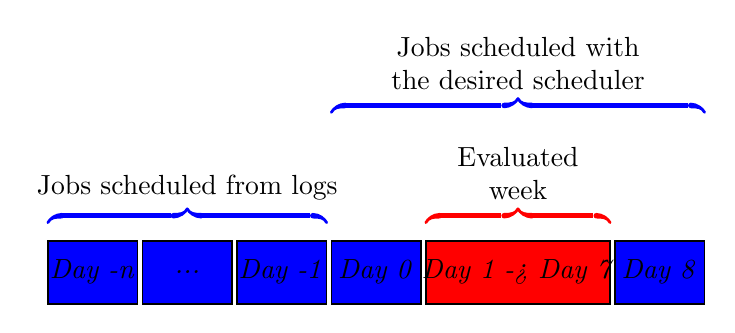
\begin{tikzpicture}[semithick, > = {Stealth[scale=1.25]}, shorten > = 1pt,]
    \def\x{1}\def\y{1}
    \draw[color=black, fill=blue] (1.2*0*\x+0.03, 0.7) rectangle (1.2*1*\x-0.03, -0.1) node[midway] {\textit{Day -n}}; 
    \draw[color=black, fill=blue] (1.2*1*\x+0.03, 0.7) rectangle (1.2*2*\x-0.03, -0.1) node[midway] {\textit{...}}; 
    \draw[color=black, fill=blue] (1.2*2*\x+0.03, 0.7) rectangle (1.2*3*\x-0.03, -0.1) node[midway] {\textit{Day -1}}; 
    \draw[color=black, fill=blue] (1.2*3*\x+0.03, 0.7) rectangle (1.2*4*\x-0.03, -0.1) node[midway] {\textit{Day 0}}; 
    \draw[color=black, fill=red] (1.2*4*\x+0.03, 0.7) rectangle (1.2*6*\x-0.03, -0.1) node[midway] {\textit{Day 1 -> Day 7}};
    \draw[color=black, fill=blue] (1.2*6*\x+0.03, 0.7) rectangle (1.2*7*\x-0.03, -0.1) node[midway] {\textit{Day 8}}; 
    \draw [pen colour={blue},decorate,line width=2pt,decoration = {calligraphic brace,raise=-2pt,amplitude=5pt}] (1.2*0*\x+0.03, 1) -- node[pos=0.5,above=2pt,black,align=center]{Jobs scheduled from logs} (1.2*3*\x-0.03, 1);
    \draw [pen colour={blue},decorate,line width=2pt,decoration = {calligraphic brace,raise=-2pt,amplitude=5pt}] (1.2*3*\x+0.03, 2.4) -- node[pos=0.5,above=2pt,black,align=center]{Jobs scheduled with\\the desired scheduler} (1.2*7*\x-0.03, 2.4);
    \draw [pen colour={red},decorate,line width=2pt,decoration = {calligraphic brace,raise=-2pt,amplitude=5pt}] (1.2*4*\x+0.03, 1) -- node[pos=0.5,above=2pt,black,align=center]{Evaluated\\week} (1.2*6*\x-0.03, 1);
  \end{tikzpicture}
}
\caption{Methodology followed to schedule and evaluate jobs from a specific week while avoiding edge effects.}\label{fig.workload}
\label{fig.ex}
\end{figure}

Our evaluation is based on three factors: the stretch of each \us, the total time spent waiting for a file to become available, as well as the total core time.
}
Our main competitors on these metrics are FCFS and EFT, with and without backfilling.

\subsection{\rev{Simulator description}}
\rev{
All strategies as well as the two baselines have been implemented
on a simulator that we developed\footnote{You can find the code and the anonymized logs of the workloads at: \url{https://github.com/userccgrid/Locality-aware-batch-scheduling}}.

The simulator is made in python and follows these principles:
\begin{itemize}
	\item The schedule is re-done entirely each time a new job is submitted or a core is liberated.
	\item The scheduler only knows the jobs whose submission time are superior or equal to the current time.
	\item The scheduler only knows the submission time, requested walltime, number of cores required and input file name of the jobs.
	\item After a schedule, each available job is associated with a start time, a node, and as many cores on that node as requested.
\end{itemize}

We didn't use an existing batch simulator like Batsim because it lacked some key elements for us, especially the ability to add a loading time for input files before starting a job or to reuse an input file already loaded on a node to skip this loading time.

We evaluated our schedulers on 12 distinct randomly selected weeks.
Among those weeks, different workload conditions can be found.
First, we study the behavior on an under-loaded cluster.
}

\subsection{\rev{Performance on an underutilized cluster}}\label{sec.40}

\begin{figure}[t]\centering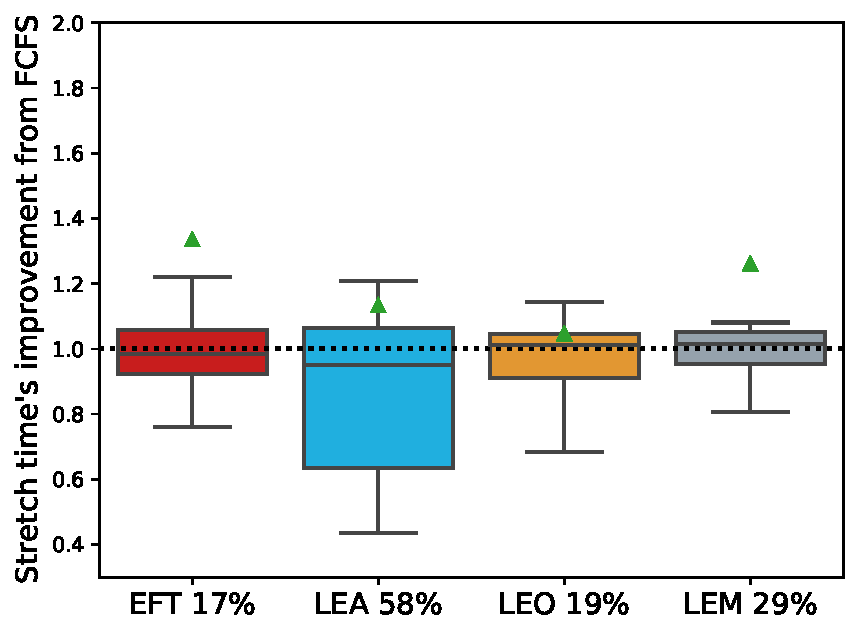
\includegraphics[width=0.9\linewidth]{../MBSS/plot/Boxplot/byuser/box_plot_stretch_10-03-10-09_0.pdf}\caption{Stretch's improvement from FCFS on week 40.}\label{stretch.40}\end{figure}

Figure~\ref{stretch.40} depicts 
\rev{
the distribution of each \us stretch's improvement compared to FCFS obtained by each strategy on week 40.
In other words it's for each \us and for each scheduler: $\frac{Stretch\_FCFS}{Stretch\_Scheduler}$.
In this figure, the horizontal black dotted line corresponds to no improvements from FCFS, which
is the situation where the sum of the queue time and transfer time of the \us is the same as with FCFS.
You can see percentages next to the scheduler names.
These are the proportion of \us where the improvement was at least 1\% different from 1.
For this boxplot only and for the sake of clarity, we are only plotting those \us on Figure~\ref{stretch.40}.
The solid line is the median and the triangle symbolizes the mean improvement. Because the outliers bring a huge improvement, the means are higher than the medians.
We care more about medians because outliers are special cases.
An improvement above 1 is a speed-up. An improvement at 0.5 means that the sum of the queue times and transfer times for this \us was two times bigger with the scheduler compared to FCFS. At 1.5 this sum was 1.5 times smaller compared to FCFS.
All the boxplot shown in this paper use octiles to draw the whiskers. 

%~ As the cluster is not very loaded in this scenario, EFT, LEO and LEM have most of their improvements close to 1. When the cluster is under-loaded, a First-Come First-Serve strategy is usually efficient because using all nodes is usually more important than re-using an input file as the duration of a job is larger than the loading time. EFT, LEO and LEM all have attributes that allows to do this.
%~ EFT takes into consideration the earliest available time, LEO changes is stratgey is the earliest available time of a node is the current time and LEM switch to EFT if all nodes are not occupied.
%~ However LEA greatly suffer from this wokload as we can see that more than 50\% of it's improvement are below 1.

From Figure~\ref{stretch.40} we learn that on this workload, all the schedulers have most of their results
around an improvement of 1 apart from LEA that has slow-downs for more than 50\% of it's results.
}

\begin{figure}[t]\centering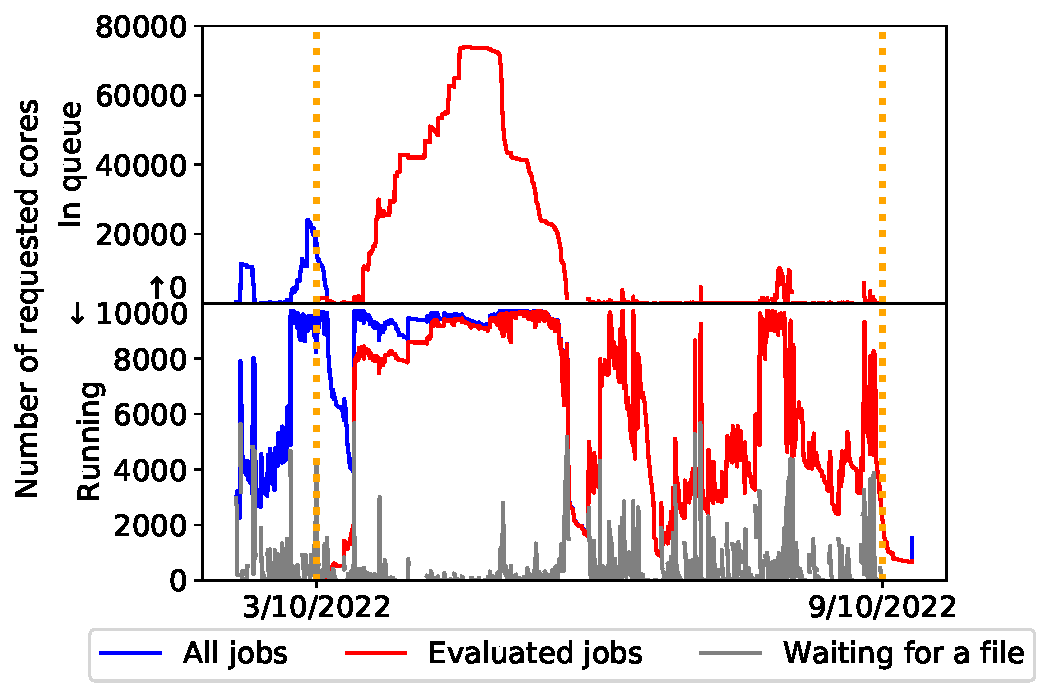
\includegraphics[width=0.9\linewidth]{../MBSS/plot/Cluster_usage/2022-10-03->2022-10-09_V10000_anonymous_Fcfs_Used_nodes_450_128_32_256_4_1024_core_by_core.pdf}\caption{Visualization of the utilization rate of the cluster on the workload of week 40 with FCFS.}\label{40_cluster_usage_fcfs}\end{figure}

To understand the issues LEA encounters on this workload, we need to study the cluster's usage over time.
Figure~\ref{40_cluster_usage_fcfs} shows the cluster usage when using FCFS.
The vertical axis represents the number of requested cores either running on a
node (lower half, \rev{here the maximum is the total number of cores on our cluster: 9720}) or in the queue of jobs waiting to be executed (top
half, \rev{here the number of requested cores can be much higher than the cluster's capability}).
The blue line shows the number of cores from all jobs.
The red lines show the number of cores used by the evaluated jobs, i.e.,
those jobs that have their submission time within our evaluation window. Thus, this forms a subset
of the set indicated by the blue line.
If a line is present in the top half, it means that some jobs could not be scheduled
and are thus waiting in the queue of available jobs. 
A node may have some available cores but not enough to accommodate some jobs with large requirements.
This explains why the waiting job queue may not be empty even if the lower half does not reach the maximum.
The gray line represents the number of cores currently loading a file.
Lastly, the orange lines delimits the submission times of our 
evaluated jobs, in other words it is our evaluation window.
By looking at the top half of Figure~\ref{40_cluster_usage_fcfs}
we understand that the job queue is empty \rev{for more than half of the evaluation window}.
In this situation, FCFS and EFT are very efficient. The earliest available node is in
most cases a node that can start the job immediately, explaining the mean stretch close to 1 in Figure~\ref{stretch.40}.
LEO is a strategy that uses the earliest available time $t_k$ of a node to decide if it should compute a score like LEA,
that puts a large weight on transfer time
or weigh equally $t_k$, the transfer and eviction duration. 
Thus, on underused clusters, LEO has a behavior close to EFT, while trying to minimize evictions.
Similarly, LEM switches between EFT and LEA depending on the cluster's usage.
On this particular workload the cluster's usage is under \rev{100\% more than half the time}, so LEM behaves similarly to EFT.
On the contrary, LEA favors data re-use over an early start time for a job.
\begin{table}
\begin{tabular}{ l c >{\columncolor{green!85}}c c c }
  \toprule
  Schedulers & EFT & LEA & LEO & LEM \\
  \midrule
  Reduction from FCFS & -0.0\% & -14.8\% & -0.8\% & -3.8\% \\ % +0.03 for EFT
  \bottomrule
\end{tabular}
\caption{Percentage reduction in time spent waiting for a file to be ready before starting the computation, relative to the total wait time of FCFS.}\label{tab.40}
\end{table}
\rev{Table~\ref{tab.40} shows the reduction from the amount of time spent 
waiting for a file to be ready before starting the computation,
relative to the total waiting time of FCFS.
In this case, LEA is the only strategy that decreases this waiting time by re-using input files.
It will create queue of jobs that already have a valid copy of their file loaded on a node, waiting to be able to re-use their input.}
On an underused cluster, this increases starvation.
The benefit of scheduling these jobs immediately on another node and loading the file appears
inferior to waiting for a file re-use for LEA and thus creates this queue of jobs that does not exist for \rev{the other schedulers}. 
\begin{figure}[t]\centering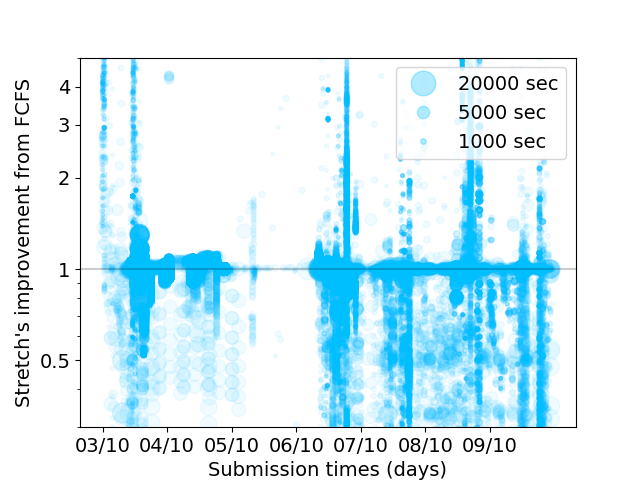
\includegraphics[width=0.9\linewidth]{../MBSS/plot/Stretch_times/Stretch_times_FCFS_LEA_2022-10-03->2022-10-09_V10000_anonymous_450_128_32_256_4_1024.png}\caption{Stretch times of each user session from week 40 using LEA compared to FCFS.}\label{40_fcfs_vs_lea}\end{figure}
\begin{figure}[t]\centering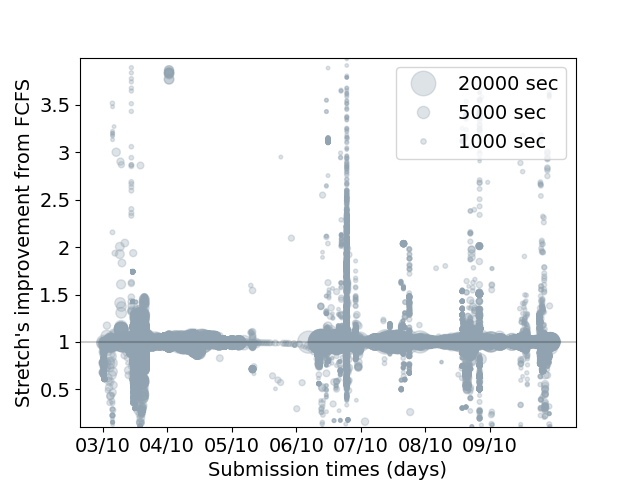
\includegraphics[width=0.9\linewidth]{../MBSS/plot/Stretch_times/Stretch_times_FCFS_LEM_2022-10-03->2022-10-09_V10000_anonymous_450_128_32_256_4_1024.png}\caption{Stretch times of each user session from week 40 using LEM compared to FCFS.}\label{40_fcfs_vs_lem}\end{figure}
The consequences for the stretch are immediately distinguishable on Figure~\ref{40_fcfs_vs_lea}.
This visualization shows for each \rev{\us}, the ratio of its stretch with LEA by its stretch with FCFS (hence a value above~1 means LEA improves the stretch).
The size of a circle is proportional to the \rev{\us's} duration.
On the workload of week~40, we observe several ``columns'' of jobs submitted at the same time (hence sharing the same file with large probability)
with a ratio lower than~1, hence a worst performance with LEA.
This means LEA is waiting to re-use the files before starting the jobs,
whereas FCFS paid the cost of loading the file on other nodes, but started the jobs
earlier than LEA, leading to shorter completion times.
From Figure~\ref{40_fcfs_vs_lem} concerning LEM, we see that most jobs have an improvement close to~1, showing 
that LEM does not fall into LEA's pathological case.

To summarize, on an underutilized cluster, LEA's focus on locality
does not allow optimal utilization of the cluster, while LEO and LEM, thanks
to their flexibility, achieve performance close to EFT.


\subsection{Results on a saturated cluster}\label{sec.43}

\begin{figure}[t]\centering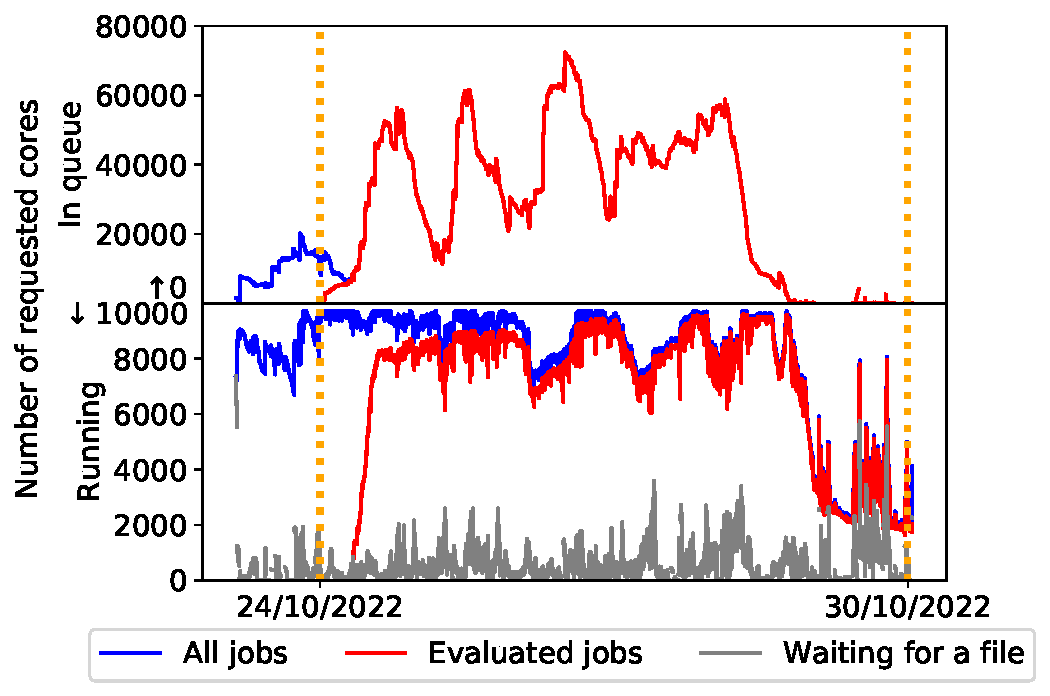
\includegraphics[width=0.9\linewidth]{../MBSS/plot/Cluster_usage/2022-10-24->2022-10-30_V10000_anonymous_Fcfs_Used_nodes_450_128_32_256_4_1024_core_by_core.pdf}\caption{Visualization of the utilization rate of the cluster on the workload of week 43 with FCFS.}\label{cluster_usage.43}\end{figure}

We study week 43. This is a workload that saturates the cluster.
Indeed, as we can see on Figure~\ref{cluster_usage.43}, there is
a queue of several thousands requested cores
for the whole duration of the evaluated \rev{week}.
In this situation, re-using files has a significant impact
on the queue times.
\rev{
\begin{figure}[t]\centering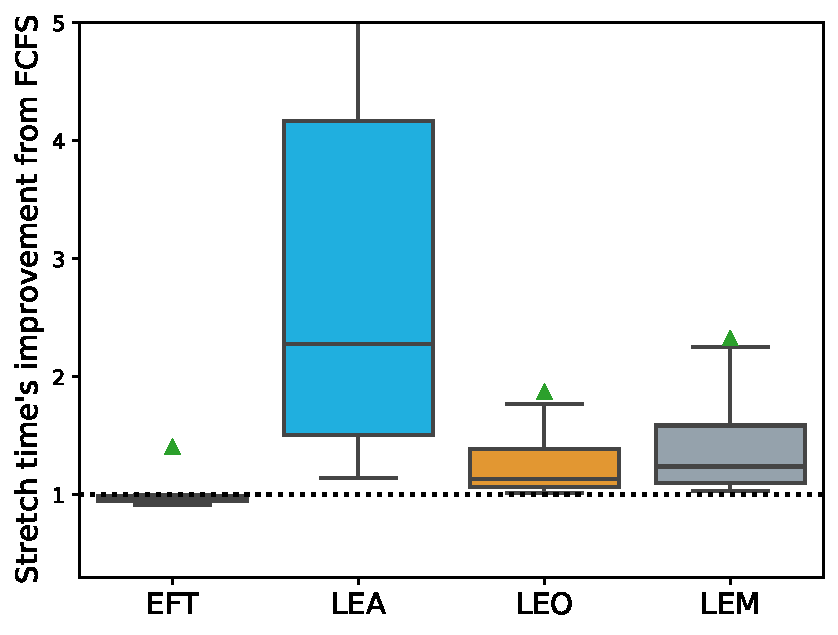
\includegraphics[width=0.9\linewidth]{../MBSS/plot/Boxplot/byuser/box_plot_stretch_10-24-10-30_1.pdf}\caption{Stretch's improvement from FCFS on week 43}\label{stretch.43}\end{figure}
\begin{table}
\begin{tabular}{ l c >{\columncolor{green!85}}c c c }
  \toprule
  Schedulers & EFT & LEA & LEO & LEM \\
  \midrule
  Reduction from FCFS & -0.4\% & -20.8\% & -1.0\% & -11.4\% \\
  \bottomrule
\end{tabular}
\caption{Percentage of reduction from the amount of time spent 
waiting for a file to be ready before starting the computation,
relative to the total waiting time of FCFS on week 43.}\label{tab.43}
\end{table}
As you can see on Table~\ref{tab.43}, LEA and LEM greatly reduces the transfer time.
}
This is confirmed by Figure~\ref{stretch.43}:
more data re-use is associated with \rev{better improvement} for LEA and LEM.
On a saturated cluster, filling all cores with the first jobs of the queue, like FCFS does, is not crucial.
It is more beneficial to group jobs using the same file.
The first few jobs have a longer queue than with FCFS,
but, over time, re-using files causes a snowball effect that reduces the
queue times of all subsequent jobs.
Moreover, the queue contains enough jobs to fill all the nodes even when grouping them by input file.
We thus avoid the pathological cases presented in \rev{section~\ref{sec.40}}.
In this case, LEA's strategy, also found in LEM, allows to greatly reduce the stretch of each \us.
\begin{figure}[t]\centering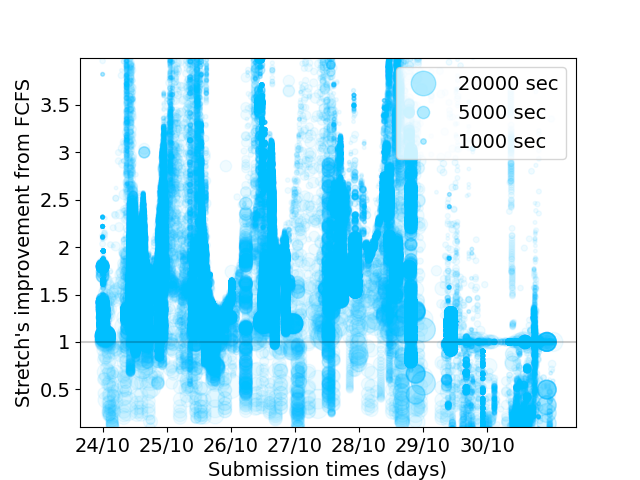
\includegraphics[width=0.9\linewidth]{../MBSS/plot/Stretch_times/Stretch_times_FCFS_LEA_2022-10-24->2022-10-30_V10000_anonymous_450_128_32_256_4_1024.png}\caption{Stretch times of each user session from week 43 using LEA compared to FCFS.}\label{vs_fcfs_lea_43}\end{figure}
We can observe this, \rev{\us by \us}, on Figure~\ref{vs_fcfs_lea_43}: very few jobs 
have a worse stretch than FCFS and a large amount of jobs are above an improvement of 2.


\subsection{\rev{Aggregated results on 12 different evaluated weeks of the workload}\todo[inline]{Max: Maybe another title would be better to say that here we have the final results?}}

We evaluated our 5 schedulers on \rev{12 different weeks}.
\rev{The Figures~9 to 12 represents the aggregated}
results of the ratio of \rev{each 136\,404 \us stretch over 12 weeks and 1\,986\,496 jobs} with the one of FCFS. 
%~ A result above the black dotted line (at~1) is thus an improvement compared to FCFS average stretch.
%~ On this figure, the box represents results within the first and the last quartile (from 25\% to 75\%, thus half of the results).
%~ The whiskers delimit the octiles (12.5\% and 87.5\%), thus 75\% of the results are contained
%~ within the whiskers. This also means that between the lower side of the box and the maximum value,
%~ we find 75\% of the results (and similarly between the upper side of the box and the minimum value).
%~ The solid green lines show the median while the dashed ones show the mean result.
%~ Each white circle is an outlier whose improvement is in the first or last octile.
%~ For better readability, 6 outliers above the upper whisker for LEA and
%~ LEM have been removed, with maximum value respectively at~33.5
%~ and~6.7.

\paragraph{\rev{Results without backfilling}}

\begin{figure}[t]\centering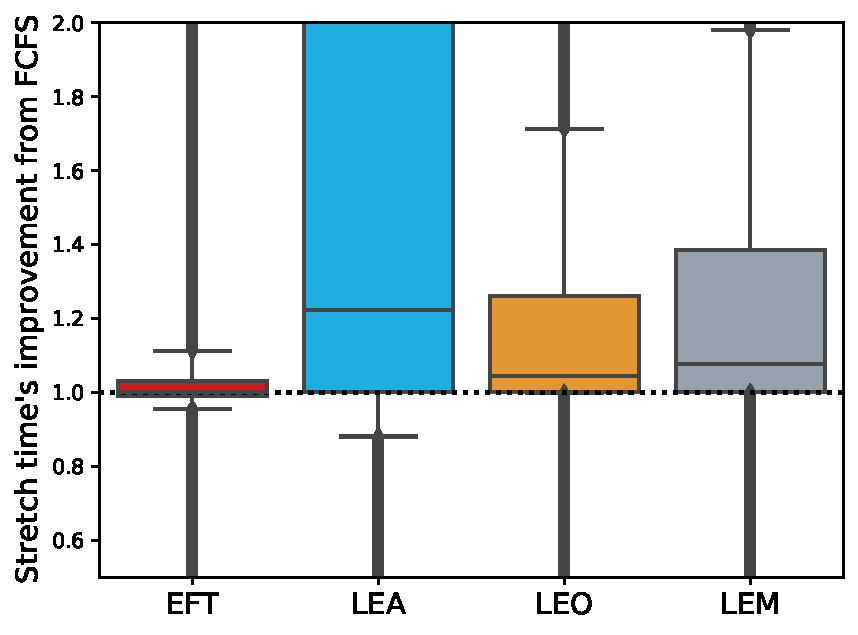
\includegraphics[width=0.9\linewidth]{../MBSS/plot/Boxplot/byuser/box_plot_stretch_all-all_1.pdf}\caption{Stretch's improvement from FCFS on all evaluated weeks.}\label{boxplot.all}\end{figure}
As in the previous results, we observe on Figure~\ref{boxplot.all} that EFT does not bring any real improvement compared to FCFS.
\rev{
\begin{table}
\begin{tabular}{ l c >{\columncolor{green!85}}c c c }
  \toprule
  Schedulers & EFT & LEA & LEO & LEM \\
  \midrule
  Reduction from FCFS & -0.9\% & -17.1\% & -0.9\% & -7.1\% \\
  \bottomrule
\end{tabular}
\caption{Percentage of reduction from the amount of time spent 
waiting for a file to be ready before starting the computation,
relative to the total waiting time of FCFS on all workloads.\todo[inline]{Max: Do we want to put green on the best one? It's always LEA on our tables.}}\label{tab.all}
\end{table}
% For LEA, LEO and LEM, the medians are respectively 1.12, 1.03 and 1.13. 
% However the mean values are much higher at 2.26, 1.21 and 1.76.
EFT takes into account file transfers when scheduling but is a less aggressive strategy than LEA or LEM, the economy in data transfers is only 0.9\% (see Table~\ref{tab.all}).
It's not able to see that a large number of jobs using the same file should be scheduled on the same node: even if it generate more queue time, the overall execution time will be lowered thanks to data re-use.
LEA has the largest median improvement.
}
We can explain the larger \rev{median} value for LEA from the good performance on heavily saturated clusters (see Section~\ref{sec.43}).
%~ In these cases, the \rev{improvements} of LEA are much higher than those of FCFS or EFT.
Re-using the same files is not detrimental to the filling of all the nodes because there are enough jobs to cover all nodes.
A large decrease \rev{(see Table~\ref{tab.all})} in the time spent waiting for a file greatly reduces the stretch of each job.
\rev{LEM has a lower median,}
however \rev{at least} 87.5\% of its results are above 1, i.e., an improvement, whereas for LEA, only approximately 75\% of the results are above 1. 
LEM is a more versatile strategy and offers higher sustained performance on non-saturated cluster at the cost
of fewer extreme improvements on heavily saturated clusters.
%~ \rev{
%~ In terms of data transfers, LEO is similar to EFT but has better improvements in terms of stretch.
%~ LEO stills orks on locality when no nodes are available, whih can lead
%~ }
\rev{
\begin{table}
\begin{tabular}{ l c >{\columncolor{green!85}}c c c }
  \toprule
  Schedulers & EFT & LEA & LEO & LEM \\
  \midrule
  Reduction from FCFS & -0.01\% & -0.37\% & -0.02\% & -0.10\% \\
  \bottomrule
\end{tabular}
\caption{Percentage of reduction of the total core time used on all workloads.}\label{tab_core.all}
\end{table}
%~ Figure~\ref{tab.all} shows us that LEA greatly reduce data transfers, as well as LEM.
%~ LEO behave similarly to EFT.
Table~\ref{tab_core.all} shows the reduction in terms of total core time (i.e. the core time on each core of each node over the 12 weeks). 
LEA reduces the total core time used. This reduction equates to 49\,000 core hours, or a reduction of 5 hours for every 20 cores of the 486 nodes over the 12 weeks.
Although it's a small percentage reduction, it can be of interest on large scale clusters that are highly demanding in terms of electrical resources.
}

\begin{figure}[t]\centering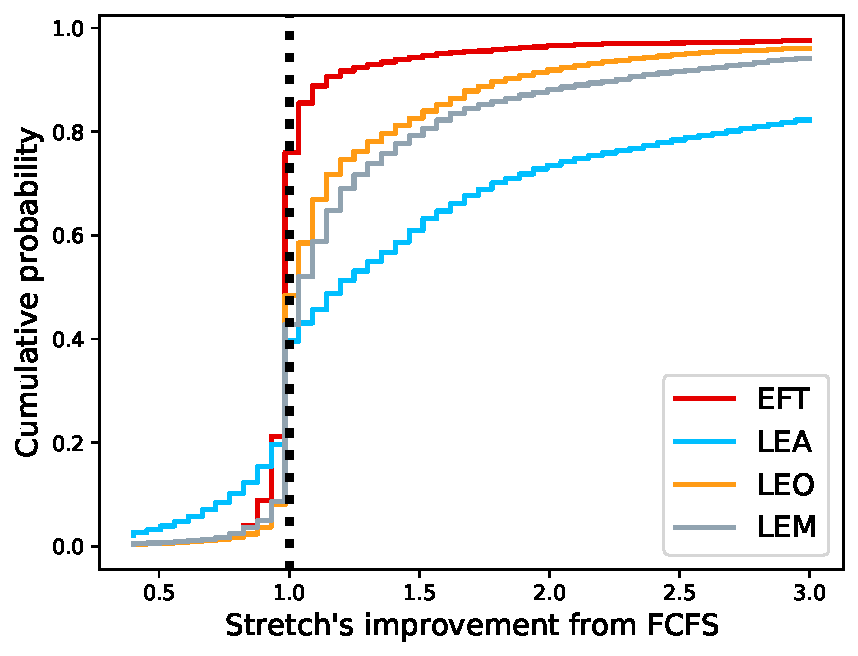
\includegraphics[width=0.9\linewidth]{../MBSS/plot/ECDF/byuser/ecdf_stretch_all-all.pdf}\caption{Empirical distribution function of the stretch's improvement from FCFS on all evaluated weeks.}\label{ecdf}\end{figure}
From the same data shown on Figure~\ref{boxplot.all}, we plot an empirical distribution function on Figure~\ref{ecdf}.
EFT's low variance is clearly visible in the sudden jump in probability around an improvement of 1.
It is interesting to note that for LEA, 20\% of the results are above an improvement of 300\%.
In addition, thanks to its switch between the strategies of EFT and LEA, LEM clearly reduces
performance losses on the left of the black line.
We can also learn from this figure that LEO is in every respect a better version of EFT \rev{as it's always under EFT after the vertical line, meaning it has more important improvements}.

Thus, without backfilling, \rev{LEA} is the best strategy to observe significant improvements.
It can compute jobs between~1 and~2 times faster in 50\% of the cases and
between~2 and~6 times faster in 25\%.
It is slower in only~25\% of the workloads, and~12.5\% of those are within a~0.15 slow-down.
LEO is a more sustained strategy with~87.5\% of its results with an improvement compared to FCFS, which shows that our opportunistic
strategy is much more consistent, while still having great improvements in some cases.
\rev{LEM achieves similar improvements}.

\paragraph{\rev{Results with backfilling}}
\begin{figure}[t]\centering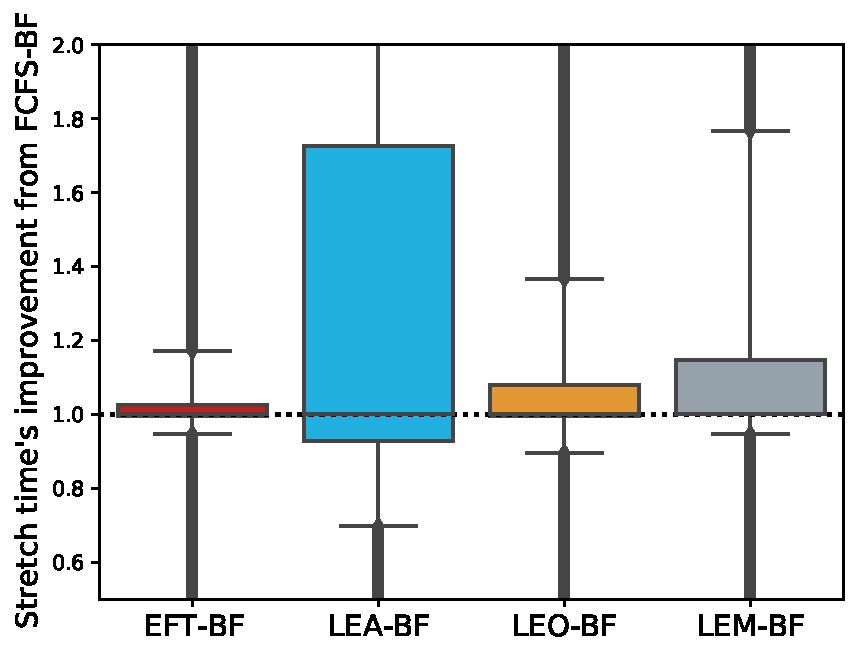
\includegraphics[width=0.9\linewidth]{../MBSS/plot/Boxplot/byuser/box_plot_bf_stretch_all-all_1.pdf}\caption{Stretch's improvement from FCFS with backfilling on all evaluated weeks.}\label{boxplot.all_bf}\end{figure}
Figure~\ref{boxplot.all_bf} shows the results with the backfilling version of our
schedulers and compared to FCFS with backfilling (FCFS-BF) on all workloads.
We notice that our schedulers have smaller improvements with backfilling.
\begin{figure}[t]\centering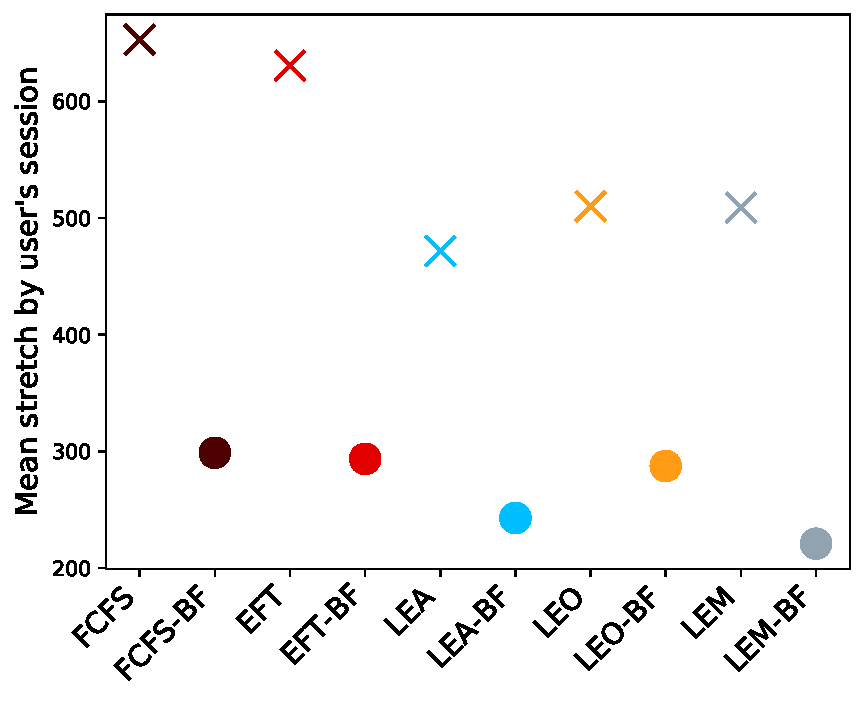
\includegraphics[width=0.9\linewidth]{../MBSS/plot/byuser/Mean_stretch_with_and_without_bf_all-all.pdf}\caption{Average stretch of all jobs evaluated on all 12 weeks by \us with (circles) and without (crosses) backfilling.}\label{bf_vs_non_bf}\end{figure}
Figure~\ref{bf_vs_non_bf} shows that
with backfilling (circles),
the \rev{difference of performance with or without backfilling is much higher} for FCFS-BF and EFT-BF. 
Our proposed strategies do not benefit from backfilling as much as FCFS-BF does for two reasons:
\begin{itemize}
	\item Even if we consider data locality when backfilling, trying to fill a node as much as possible and optimizing data re-use are two contrary goals. 
	Backfilling a job can compromise a re-use pattern that was planned by our locality-aware strategy, thus reducing the total 
	amount of re-used files.
	\item Our strategies are already able to nicely fill the nodes without needing backfilling.
	Grouping jobs by input file implies that similar jobs end up on the same nodes.
	Jobs having the same duration and number of requested cores can much more easily fill a node to its fullest than a completely heterogeneous set of jobs.
	Consequently, the shortfall without backfilling is much lower for LEA-BF, LEO-BF and LEM-BF, than for FCFS-BF and EFT-BF.
\end{itemize}
Compared to FCFS-BF, our strategies still reduce the total queue time with backfilling but the difference is less significant.

Figure~\ref{boxplot.all_bf} shows that the improvement of EFT-BF compared to FCFS-BF is not significant.
%~ LEA-BF has a median \rev{on 1}. However it still achieves a better average result.
Out of our four heuristics, LEM-BF is the best compromise \rev{here}.
It is better than FCFS-BF in more than 75\% of the cases, 
with 12.5\% of those results above an improvement of~1.8.
Among the slow-downs, only 12.5\% are superior to 0.05.

\section{Conclusion}\label{sec.conclusion}

Batch schedulers are key components of computing clusters, and aim at
improving resource utilization as well as decreasing jobs' response
time. We have studied how one may improve their performance by taking
job input file into account: in clusters dedicated to data analysis,
users commonly submit dozens jobs using the same multi-GB input
file. Classical job schedulers are unaware of data locality and thus
fail to re-use data on nodes. We have proposed three new locality-aware
strategies, named LEA, LEO and LEM,
capable of increasing data locality by grouping together 
jobs sharing inputs. The first one has a major focus on data locality,
while the other two target a balance between data locality and load
balancing. We have performed simulations on logs of an actual
cluster. Our results show that \rev{LEA} significantly improves the mean
waiting time of a job, especially  
when the cluster is under a high computing demand.
Without backfilling, \rev{LEA} is better than our baseline in 75\% of the
cases (50\% of the cases with backfilling).
\rev{Our strategy called LEM is the best compromise. It's better than the baseline in more than 75\% of the cases with or without backfilling.}

This work opens several exciting future directions.
Firstly, LEM can be tuned to better adapt to the utilization rate of the cluster.
Switching between a locality first and distribution first strategy could be done 
gradually.
Secondly, we saw that LEO was very resilient but did not re-use enough the files to provide significant improvements.
%~ \rev{Thirdly,} we could improve the pairing of backfilling and file re-use.
\rev{
An extension towards workflow scheduling where tasks depend on the output of a previous task would be great.
Indeed the output file in memory would be re-usable for other jobs, which is a 
new opportunity for locality-aware schedulers.
In the long run, our objective is to consider others issues raised by batch scheduling like
improving fairness between users, or dealing with advance reservations.
Lastly, we want to implement our strategies on the real cluster
to test their robustness in real-world situations.
}

\bibliographystyle{acm}
\bibliography{ref.bib}
\end{document}
